\documentclass[tikz,border=8pt]{standalone}
\usepackage{amsmath,amssymb}
\usetikzlibrary{arrows.meta,calc,decorations.markings,decorations.pathmorphing,patterns,shapes.geometric,positioning}

\begin{document}
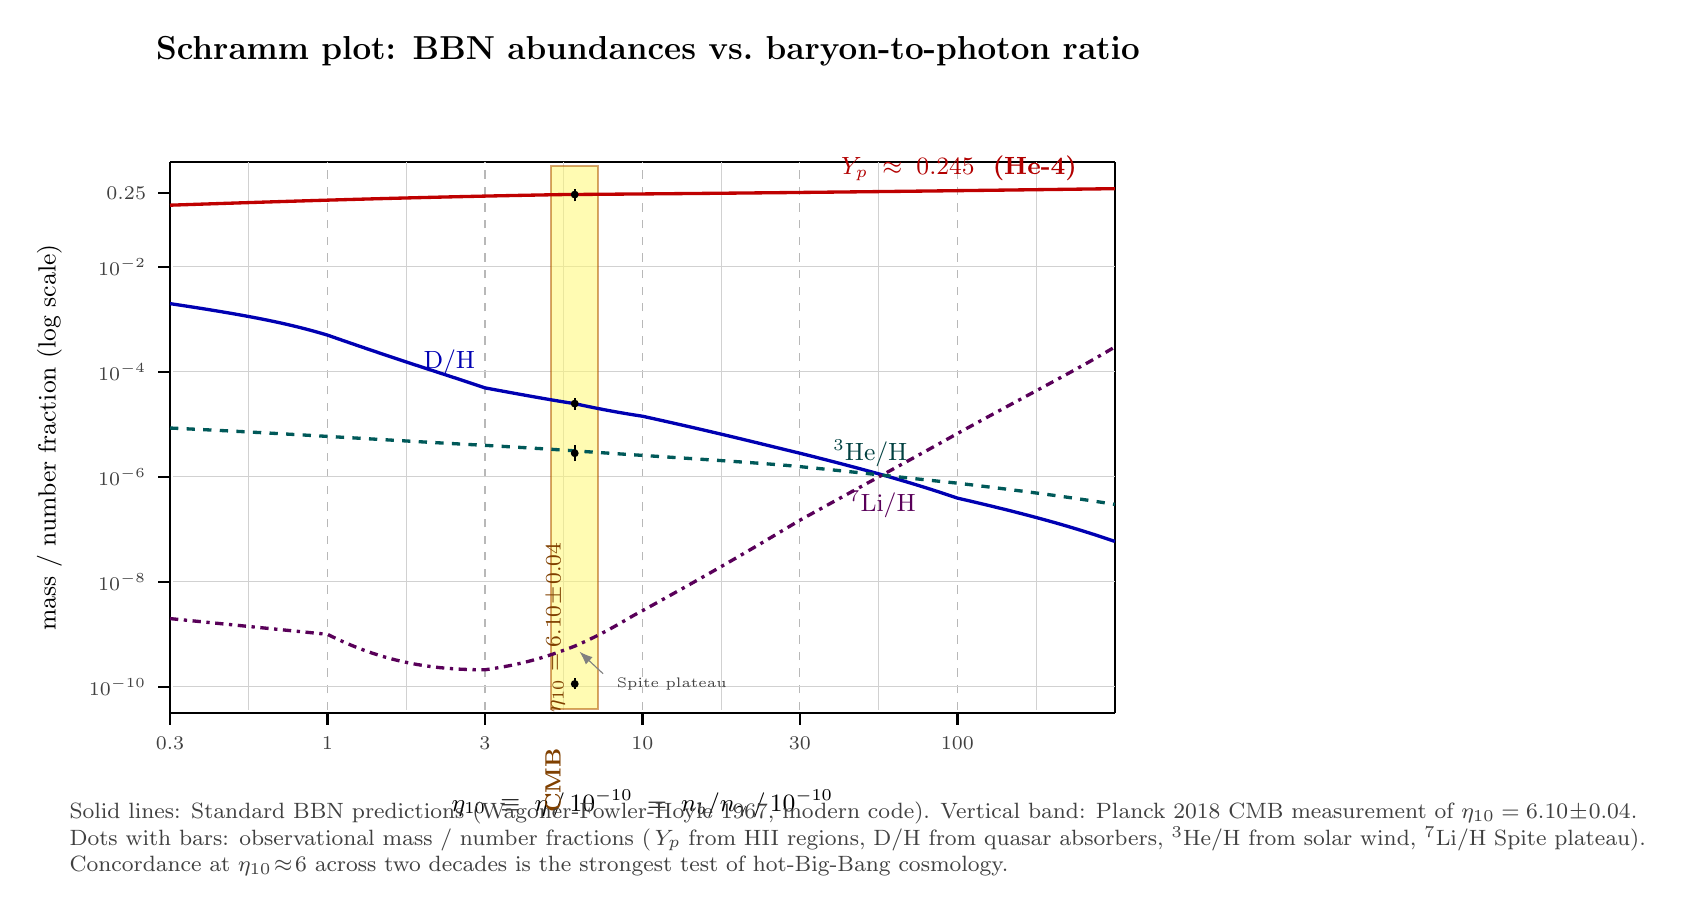
\begin{tikzpicture}[>=Latex,
  axisline/.style={draw=black, thick},
  ticklbl/.style={font=\scriptsize, text=black!75},
  axislbl/.style={font=\small},
  curveHe/.style={draw=red!75!black, very thick},
  curveD/.style={draw=blue!70!black, very thick},
  curveHe3/.style={draw=teal!70!black, very thick, dashed},
  curveLi/.style={draw=violet!70!black, very thick, dash dot},
  cmbband/.style={fill=yellow!55, draw=orange!70!black, thick, opacity=0.55},
  datapt/.style={circle, fill=black, draw=black, inner sep=0pt, minimum size=2.4pt},
  errbar/.style={draw=black, thick}]

  % --- Title ---------------------------------------------------------------
  \node[font=\large\bfseries, anchor=west] at (-0.3, 8.4)
    {Schramm plot: BBN abundances vs.\ baryon-to-photon ratio};

  % ===== AXES =============================================================
  % Plot box: x in [0, 12]   (data units: log10(eta/1e-10) from -1 to 2)
  %           y in [0, 6.6] (data units: log10(mass fraction) from -10.5 to 0)
  % We map: data_x in [-1, 2]  -> plot_x in [0, 12]   (4 units per decade)
  %         data_y in [-10.5,0]-> plot_y in [0, 6.6]  (0.6286 units per decade up; we use 6.3 height)
  % For simplicity we just place by hand using approximate normalized coordinates.

  \draw[axisline] (0, 0) -- (12, 0);          % x axis
  \draw[axisline] (0, 0) -- (0, 7.0);          % y axis
  \draw[axisline] (12, 0) -- (12, 7.0);        % right border
  \draw[axisline] (0, 7.0) -- (12, 7.0);       % top border

  % --- X axis: log eta in 10^-10 -----------------------------------------
  % decade marks at eta = 0.1, 1, 10, 100  (i.e. 10^-11 ... 10^-8 baryon/photon)
  % But the standard Schramm plot is from eta=1 to eta=10 in units of 10^-10
  % We span eta = 10^-10.5 to 10^-8.5  -> i.e. 0.32 to 32 in units of 1e-10.
  % Position: log10(eta_10) ranges -0.5 to 1.5; plot_x = 4*(log10+0.5).
  % Major ticks at eta_10 = 1, 3, 10, 30
  \foreach \loge/\xpos/\lbl in {-0.5/0/{0.3}, 0/2/{1}, 0.5/4/{3}, 1/6/{10}, 1.5/8/{30}, 2/10/{100}} {
    \draw[axisline] (\xpos, 0) -- (\xpos, -0.15);
    \node[ticklbl, anchor=north] at (\xpos, -0.18) {\lbl};
  }
  % minor x grid (decades)
  \foreach \xpos in {1, 3, 5, 7, 9, 11} {
    \draw[draw=black!18, thin] (\xpos, 0.04) -- (\xpos, 7.0);
  }
  \foreach \xpos in {2, 4, 6, 8, 10} {
    \draw[draw=black!28, thin, dashed] (\xpos, 0.04) -- (\xpos, 7.0);
  }

  \node[axislbl, anchor=north] at (6, -0.85) {$\eta_{10}\;\equiv\;\eta\,/\,10^{-10}\;=\;n_b/n_\gamma\,/\,10^{-10}$};

  % --- Y axis: mass fraction (log) ---------------------------------------
  % Range log10(X) from -10.5 to 0, plot_y from 0 to 7.0
  % scale: plot_y = (logX + 10.5) * 7.0 / 10.5  =  (logX + 10.5) * 0.6667
  \foreach \logy/\ypos/\lbl in {-10/0.333/{$10^{-10}$}, -8/1.667/{$10^{-8}$}, -6/3.0/{$10^{-6}$}, -4/4.333/{$10^{-4}$}, -2/5.667/{$10^{-2}$}, -0.6/6.6/{$0.25$}} {
    \draw[axisline] (0, \ypos) -- (-0.15, \ypos);
    \node[ticklbl, anchor=east] at (-0.18, \ypos) {\lbl};
  }
  % horizontal faint grid
  \foreach \ypos in {0.333, 1.667, 3.0, 4.333, 5.667} {
    \draw[draw=black!18, thin] (0.04, \ypos) -- (12, \ypos);
  }
  \node[axislbl, rotate=90, anchor=south] at (-1.25, 3.5) {mass / number fraction (log scale)};

  % ===== CMB measurement band ============================================
  % eta_10 = 6.1 (Planck CMB), with width approx +-0.5
  % log10(6.1) = 0.785;  log10(5.6) = 0.748;  log10(6.6) = 0.820
  % plot_x = 4*(log10+0.5) = 5.14 center;   half-width approx 0.30
  \fill[cmbband] (4.84, 0.05) rectangle (5.44, 6.95);
  \node[font=\footnotesize\bfseries, anchor=south, align=center, rotate=90, text=orange!50!black]
    at (5.14, 0.45) {CMB \quad $\eta_{10}=6.10\!\pm\!0.04$};

  % ===== CURVE: He-4 (Y_p) ============================================
  % Y_p ranges from ~0.22 at eta_10=1 to ~0.25 at eta_10=10
  % log10(Y_p) ~ -0.66 nearly flat (very weak slope)
  % plot_y = (logX + 10.5) * 0.6667
  % logX = -0.66 -> plot_y = 6.56
  % Curve nearly flat at top
  \draw[curveHe]
       (0,    6.45)
    .. controls (1.5,6.50) and (3.0,6.55) ..
       (5.0,  6.585)
    .. controls (7.0,6.60) and (9.0,6.62) ..
       (12,   6.66);

  % ===== CURVE: D/H ============================================
  % D/H drops sharply with increasing eta:
  % at eta_10 = 1, D/H ~ 5e-4; at eta_10=6, D/H ~ 2.5e-5; at eta_10=30, D/H ~ 1e-6
  % positions (data x, log10 D/H):
  % x=0(eta=0.3)/logX=-2.7  -> y= 5.20
  % x=2(eta=1)/logX=-3.30  -> y = 4.80
  % x=4(eta=3)/logX=-4.30  -> y = 4.13
  % x=5.14(eta=6.1)/logX=-4.60 -> y = 3.93
  % x=6(eta=10)/logX=-4.85 -> y = 3.77
  % x=8(eta=30)/logX=-5.55 -> y = 3.30
  % x=10(eta=100)/logX=-6.40 -> y = 2.73
  \draw[curveD]
       (0,    5.20)
    .. controls (1.0, 5.05) and (1.5, 4.95) ..
       (2.0,  4.80)
    .. controls (3.0, 4.45) and (3.5, 4.30) ..
       (4.0,  4.13)
    .. controls (4.7, 4.00) and (5.0, 3.95) ..
       (5.14, 3.93)
    .. controls (5.5, 3.85) and (5.8, 3.80) ..
       (6.0,  3.77)
    .. controls (7.0, 3.55) and (7.5, 3.42) ..
       (8.0,  3.30)
    .. controls (9.0, 3.05) and (9.5, 2.90) ..
       (10.0, 2.73)
    .. controls (11.0, 2.50) and (11.5, 2.35) ..
       (12.0, 2.18);

  % ===== CURVE: He-3 / H ============================================
  % Roughly flat, around 1e-5; weak slope.
  % He-3 / H ~ 1.5e-5 at eta=1, ~1e-5 at eta=6, ~5e-6 at eta=30
  \draw[curveHe3]
       (0,    3.62)        % logX ~ -5.07
    .. controls (1.5, 3.55) and (2.5, 3.48) ..
       (4.0,  3.40)
    .. controls (4.7, 3.36) and (5.0, 3.34) ..
       (5.14, 3.33)
    .. controls (6.0, 3.27) and (7.5, 3.18) ..
       (8.0,  3.13)
    .. controls (9.0, 3.03) and (9.5, 2.97) ..
       (10.0, 2.92)
    .. controls (11.0, 2.80) and (11.5, 2.73) ..
       (12.0, 2.65);

  % ===== CURVE: Li-7 / H (valley shape) ============================
  % Li-7 / H ~ 1e-9 at eta=1, drops to 1.5e-10 at eta~3, rises again to ~1e-9 at eta=10, ~1e-7 at eta=100
  % logX values: -9, -9.8, -9, -7
  \draw[curveLi]
       (0,    1.20)        % logX ~ -8.7
    .. controls (1.0, 1.10) and (1.5, 1.05) ..
       (2.0,  1.00)        % eta=1, logX=-9
    .. controls (2.7, 0.65) and (3.3, 0.55) ..
       (4.0,  0.55)        % eta=3, logX=-9.7 (valley)
    .. controls (4.5, 0.62) and (4.8, 0.72) ..
       (5.14, 0.85)        % CMB pos
    .. controls (5.6, 1.05) and (5.8, 1.20) ..
       (6.0,  1.30)        % eta=10
    .. controls (7.0, 1.85) and (7.5, 2.15) ..
       (8.0,  2.45)
    .. controls (9.0, 3.00) and (9.5, 3.27) ..
       (10.0, 3.55)
    .. controls (11.0, 4.10) and (11.5, 4.35) ..
       (12.0, 4.65);

  % ===== Curve labels =========================================
  % Helium-4 label - near the top
  \node[font=\small\bfseries, text=red!70!black, anchor=west]
    at (8.4, 6.92) {$Y_p\;\approx\;0.245$ \;(He-4)};

  % D/H label
  \node[font=\small, text=blue!70!black, anchor=east]
    at (4.0, 4.45) {D/H};

  % He-3/H label
  \node[font=\small, text=teal!50!black, anchor=west]
    at (8.3, 3.30) {$^3$He/H};

  % Li-7/H label
  \node[font=\small, text=violet!70!black, anchor=west]
    at (8.5, 2.65) {$^7$Li/H};

  % ===== Data points (with error bars) =====================
  % He-4:  Y_p_obs = 0.245 (Aver et al.) at eta_10 ~ 6
  \draw[errbar] (5.14, 6.50) -- (5.14, 6.66);
  \node[datapt] at (5.14, 6.585) {};

  % D/H: deuterium (Cooke 2018) D/H = (2.527+-0.030)e-5 -> log = -4.597 -> y = 3.94
  \draw[errbar] (5.14, 3.85) -- (5.14, 4.00);
  \node[datapt] at (5.14, 3.93) {};

  % He-3/H solar wind ~ 1.5e-5
  \draw[errbar] (5.14, 3.20) -- (5.14, 3.40);
  \node[datapt] at (5.14, 3.30) {};

  % Li-7/H Spite plateau: log(Li/H) ~ -9.94 -> y = 0.37 (lower than predicted)
  % Predicted at CMB band: y = 0.85; observed y = 0.37. Show observed point.
  \draw[errbar] (5.14, 0.30) -- (5.14, 0.45);
  \node[datapt] at (5.14, 0.37) {};
  \node[font=\tiny, text=black!75, anchor=west, align=left]
    at (5.55, 0.37) {Spite plateau};
  \draw[->, thin, gray] (5.50, 0.50) -- (5.20, 0.78);

  % ===== Bottom legend =====================================
  \node[font=\footnotesize, anchor=west, align=left, text=black!75]
    at (-1.4, -1.6)
    {Solid lines: Standard BBN predictions (Wagoner-Fowler-Hoyle 1967, modern code).
     Vertical band: Planck 2018 CMB measurement of $\eta_{10}=6.10\!\pm\!0.04$.\\
     Dots with bars: observational mass / number fractions (\,$Y_p$ from HII regions, D/H from
     quasar absorbers, $^3$He/H from solar wind, $^7$Li/H Spite plateau).\\
     Concordance at $\eta_{10}\!\approx\!6$ across two decades is the strongest test of hot-Big-Bang
     cosmology.};

\end{tikzpicture}
\end{document}
